% TODO:
% Better picture of HC-05?
% Update architecture PNG - Are we including PI talks to PI?
% Architecture figure to different section
% 'IoT' or 'Internet of Things'? need to define IoT earlier!
% Mention outreach? - perhaps to introduce the graph section
% Sort out topics!
% - What is broker-services/hello?
% - Don't post the time in the last will
% - Order of time and status
% Ensure that what is written here about Bluetooth working with our setup if a set of devices is provided is correct
% Sort out tenses
% Confirm 'suffix' is a correct term for final topic in MQTT?
% The section on broker services shouldn't live under protocols


We implemented a test bed for future development of an Internet of Things security protocol. Our proof-of-concept used standard IoT components to produce a system that moved data over the different levels of our architecture, demonstrating common features of a large scale infrastructure.


% ✔ We wanted to make a prototype for use as a test bed (or proof-of-concept) for future development of an IoT security protocol, blah.
% Also used for outreach activities, blah
% ✔ Chose to use off-the-shelf component for maximum applicability, blah


\subsection{Equipment}
\paragraph{}
For Edge Devices, we used Arduino Unos which are inexpensive (£25-30), low powered and portable making them a popular choice for use with IoT. With 14 inputs and outputs (analog and digital), these microcontrollers can be loaded with pre-compiled programs to interact with sensors. To communicate with Smart Agents, we used Serial over either USB or Bluetooth (through the addition of a HC-05 Bluetooth module - see Figure \ref{fig:HC-05}).


\begin{figure}
    \centering
    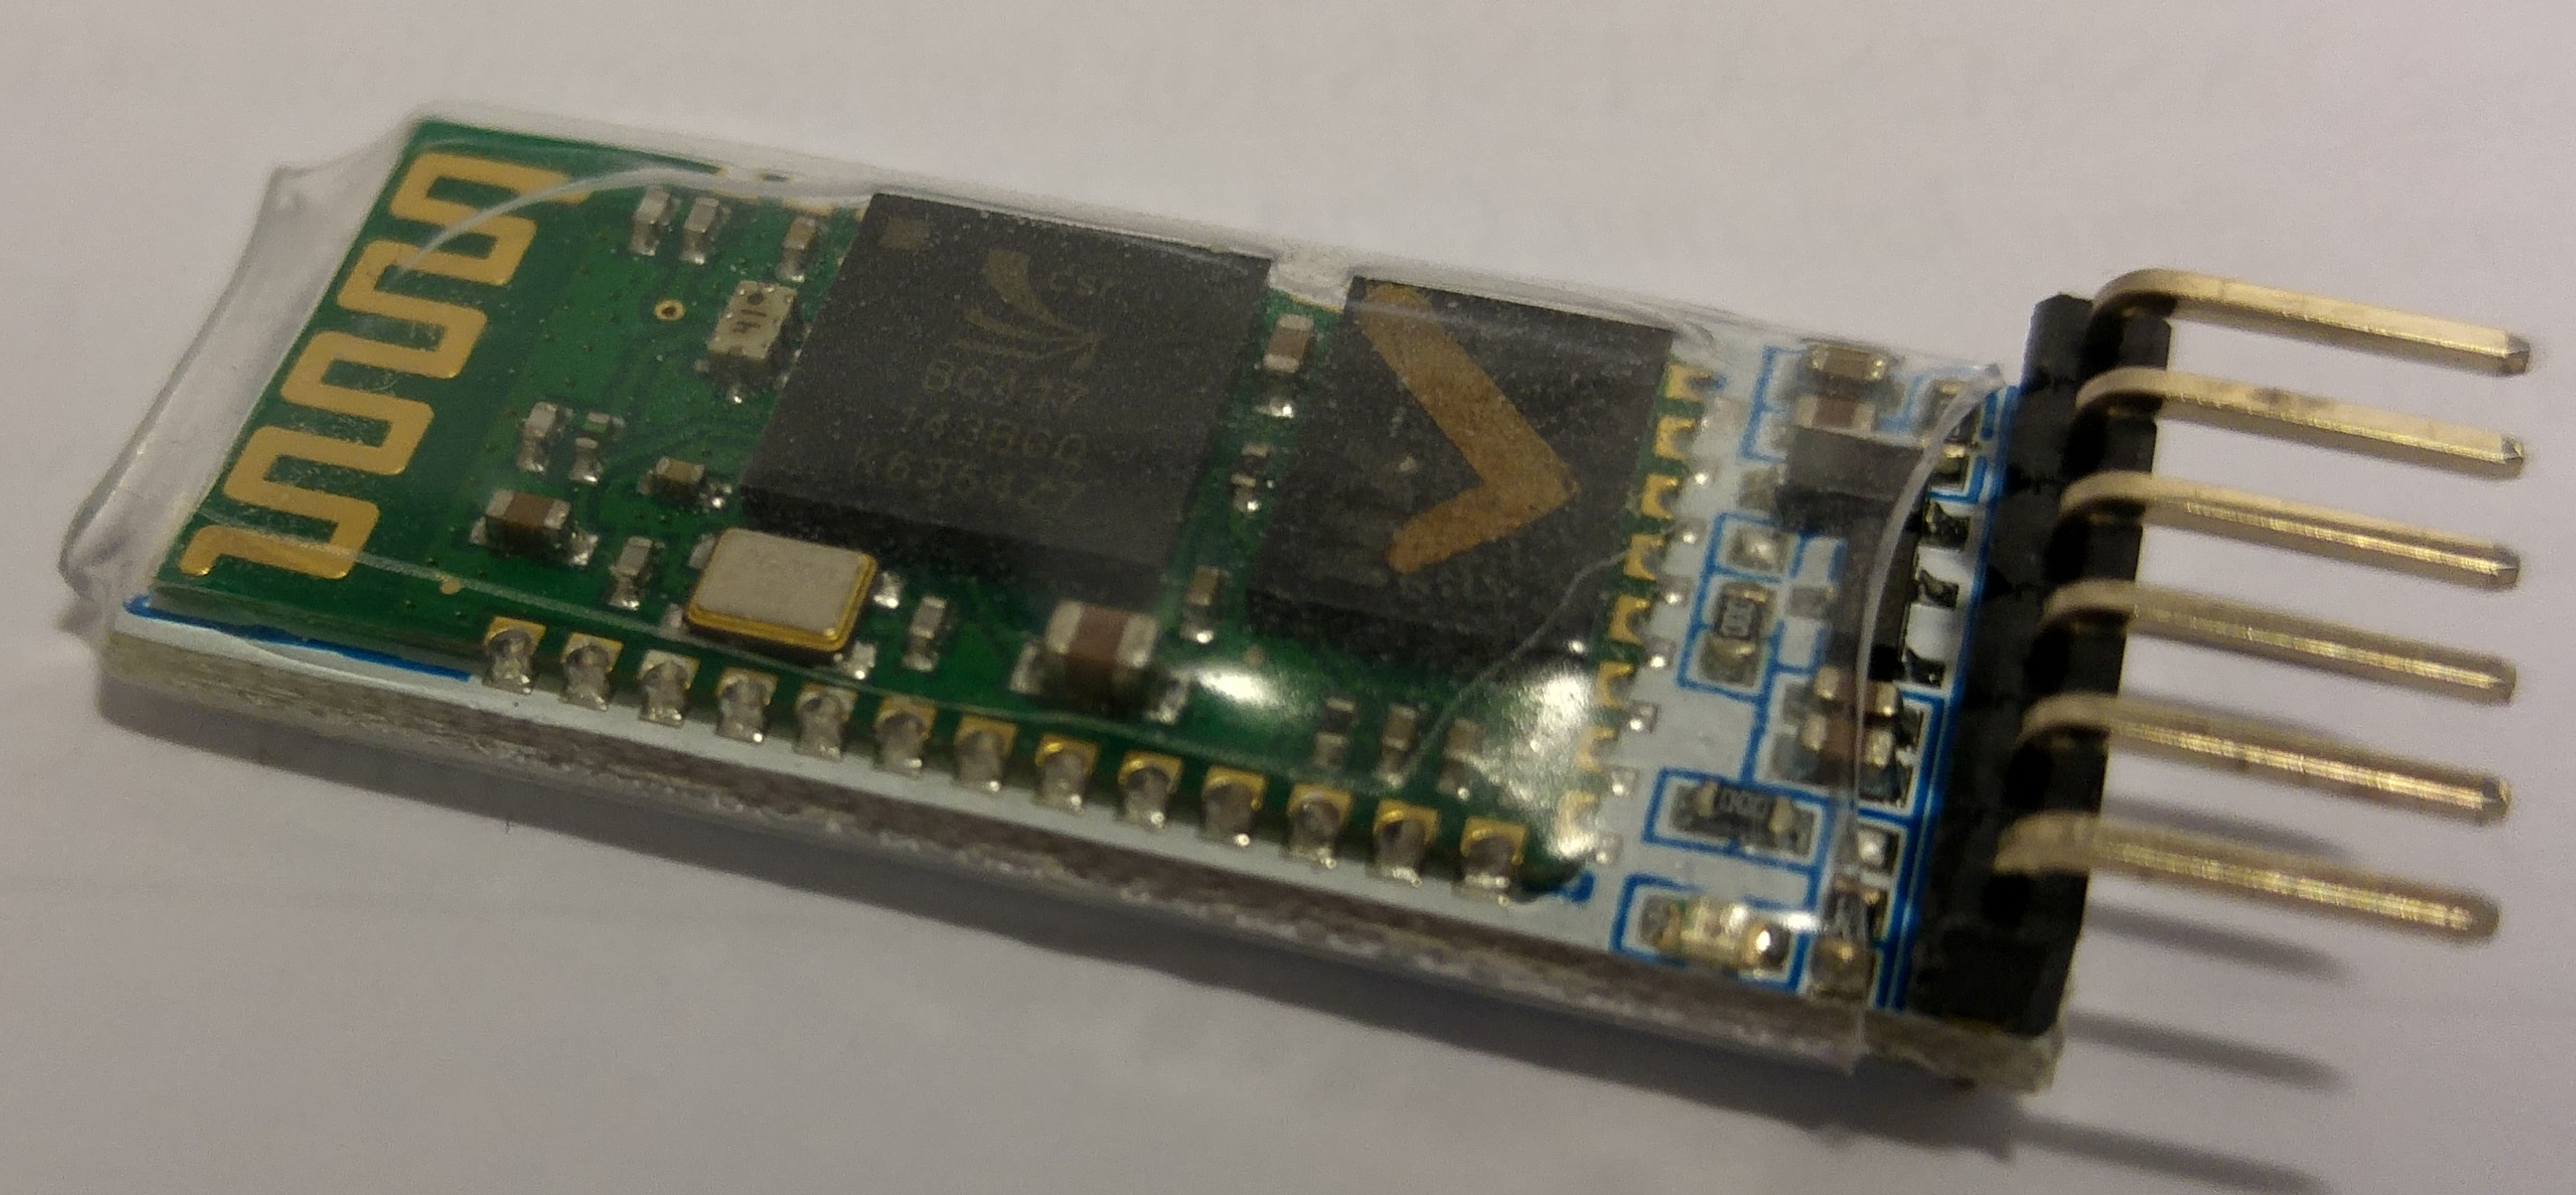
\includegraphics[width=0.5\textwidth]{HC05.jpg}
    \caption{The HC-05 chip for serial over Bluetooth. It costs roughly £4 and has a range of about 10m. Requiring a pin to pair the devices, it can have the role of either slave (wait for connection) or master (search for device to connect to).}
    \label{fig:HC-05}
\end{figure}

\paragraph{}
As Smart Agents, we used the Raspberry PI 3 which is a single board computer. Communication with Edge Devices and the Cloud was possible over USB, Ethernet, WiFi and Bluetooth without any additional adapters. The PI can run PC scale applications headless on its Linux operating system. Its low price, small form factor and low power requirement make it popular for IoT.

\paragraph{}
We used STFC's SCD Cloud for access to a virtual machine running Scientific Linux 7. A common LAN enabled TCP/IP communication between this machine and the Smart Agents or the viewer of the web application.

% ✔ We used Arduino Unos (£25-30) as edge devices. They have X inputs and outputs (analog and digital) and can be loaded with pre-compiled programs.
% ✔ HC-05 chip for Bluetooth option (picture of HC-05, range=10m?, cost=£4...)
% ✔ Raspberry pi as smart agents. Stats – 1GB RAM, can be run headless, use linux...
% ✔ SCD Cloud machine (Scientific Linux 7) hugely useful, blah.

\subsection{Setup}

\begin{figure}
    \centering
    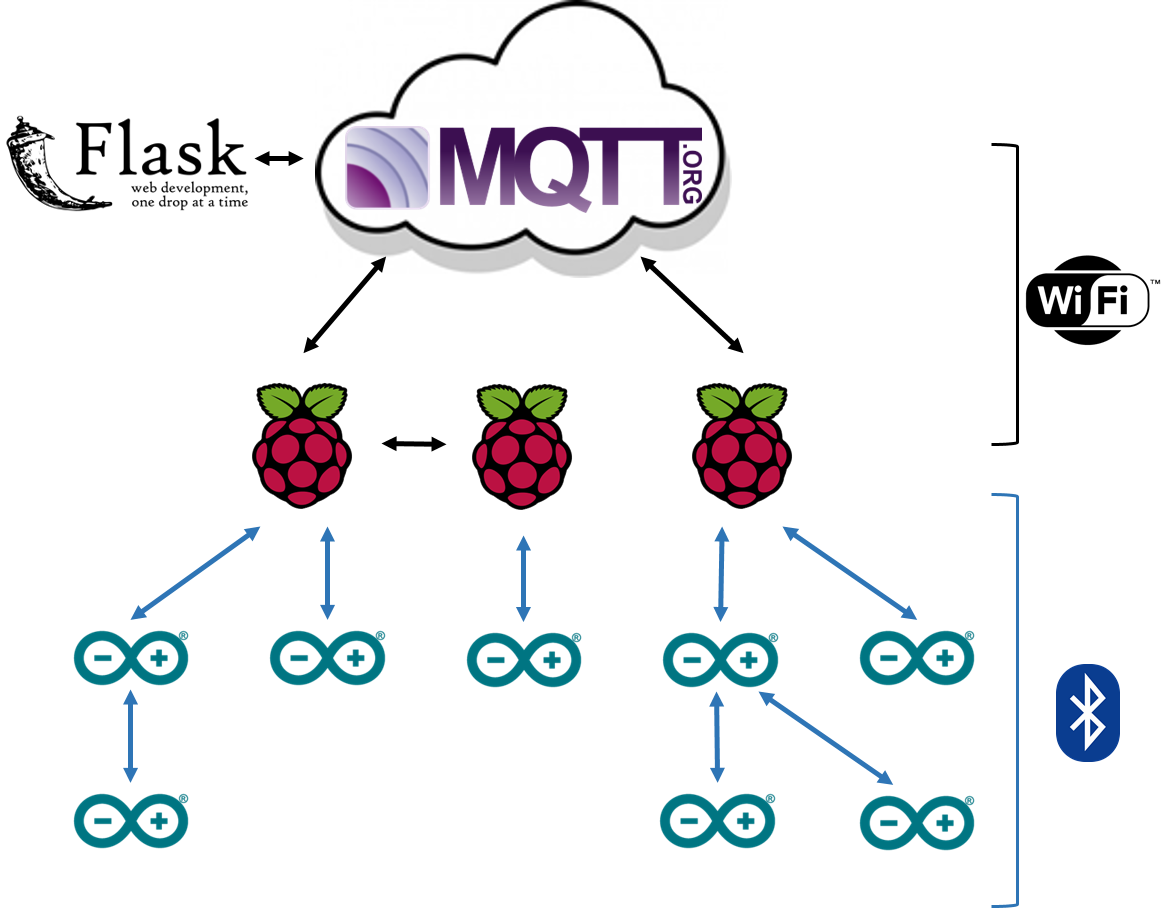
\includegraphics[width=0.5\textwidth]{Architecture.png}
    \caption{The architecture}
    \label{fig:architecture}
\end{figure}

\paragraph{}
The Cloud VM was setup as the MQTT broker using Mosquitto. There were three endpoints contacting it: Smart Agents, Broker Services and the web application. Using the Paho MQTT client library for Python, the Smart Agents acted as a gateway to the Cloud for any connected Edge Devices. Broker Services ran on the Cloud as a Python application (also using Paho) to publish a list of currently connected devices for discovery. Using a Flask module (Flask-MQTT) to serve a web application, a user could subscribe to topics for an overview of the data flows in the network.

\paragraph{}
A Smart Agent could have up to seven Edge Devices in a Bluetooth piconet. The agent scanned for a name matching a predefined pattern and then attempted to connect. However, with only one Bluetooth chip, each PI could not send/receive while scanning so communications experienced a substantial delay (roughly 20s). To counter this, we used a fixed list of Edge Devices per Smart Agent which were always available. While seemingly restrictive, this would work adequately for a variety of use cases - such as a central Smart Agent controlling statically placed sensors in a house or vehicle. Alternatively, the serial protocol worked over USB where Edge device connection was detected without interupting communication but was not wireless.

% ✔ Each edge device is identified by a unique ID which is a random number
% ✔ Communication between Smart Agent and Edge via Bluetooth.
% What is Bluetooth /why is it a good option for communicating with low memory/power/connectivity devices? PAIRING!
% ✔ Smart agents run Piduino to interface between MQTT Pub/Sub and the inputs and outputs in the edge
% ✔ Broker (mosquitto) runs on cloud, as does telemetry and monitoring applications (broker services) and a flask app.
% Pretty diagrams and pictures of the equipment
% ✔ Diagram with the pretty logos on it I made for the pre-coffee talk. I’ll go find it. The programming

\subsection{Protocols}

There were protocols for connection, normal operation and disconnection.

\paragraph{} % Connection
The connection protocol consisted of establishing a unique id and publishing it to make other devices aware. Our Smart Agents were hardcoded with a unique identification string referred to as \verb|AgentName| - the base topic for communication. On connection to the broker, each Smart Agent published 'C' to \verb|AgentName/private/status|. As each Edge Device connected, the Smart Agent initiated a handshake protocol to prompt the new device to send the random number it generated for its id on start-up. This id was then appended to a list which is encoded as JSON and published on the broker under \verb|AgentName/private/edge|. Updates to these two topics were made using retained messages so that the most up to date information was immediately sent to each new subscriber.

\paragraph{} % Normal operation
During normal operation, the Smart Agent acted as a sophisticated gateway for the Edge Devices to communicate with the Cloud. It subscribed to \verb|AgentName/public/EdgeId/output/outputName| for each \verb|EdgeId| of its Edge Devices. The suffix (\verb|outputName|) refers to a specific output attached to that Edge Device (e.g. an LED). It took any message it receives on these topics and sends a package of \verb|outputName| and the message payload to the specific Edge Device. For example if it received a payload of '1' on \verb|AgentName/public/EdgeId/output/buzzer| it sent a message instructing the Edge Device to turn on the buzzer. Similarly, when the Edge Device sent data packaged with a data value and a \verb|sensorName|, the Smart Agent published this data under \verb|AgentName/public/EdgeId/input/sensorName|.

\paragraph{} % Disconnection
There were two types of Smart Agent disconnections: graceful and ungraceful. The disconnection protocols began after initial connection to the broker when the Smart Agent set its last will as 'DU' on the status topic. This meant that if the socket to the broker closed unexpectedly, then the broker would update the agent's status to show an ungraceful disconnection. Alternatively, if the Smart Agent intended to disconnect (for example before shutdown) then it posted 'DG' to the status topic. As with connection, these were set as retained messages.

\paragraph{} % Broker Services
Broker Services subscribed to the status topic of each of the Smart Agent and maintained a central list of those which were currently available. It published the list as JSON on \verb|broker-services/discovery| with a retained message, making it easy to discover devices on the network. While the application ran on the Cloud server for convenience, this was unnecessary as it could have run from anywhere with network connection to the broker. The functionality could also be imported as a module, enabling any Smart Agent to track the available agents without depending on the central instance (although it would have to subscribe and process individual status updates from all Smart Agents).

\begin{center}
    \begin{table}
        \begin{tabular}{ | l | p{7cm} |}
        \hline
        Key Topic & Description of Content \\ \hline
        broker-services/discover & Broker Services maintains a list of currently connected devices here as a retained message.\\ \hline
        AgentName/public/EdgeId/input/sensorName & Data collected from \verb|sensorName| by \verb|EdgeId| connected to \verb|AgentName| \\ \hline
        AgentName/public/EdgeId/output/outputName & Commands sent to \verb|outputName| by \verb|EdgeId| connected to \verb|AgentName| \\ \hline
        AgentName/private/log & Debugging information for \verb|AgentName| \\ \hline
        AgentName/private/error & Debugging information for \verb|AgentName| \\ \hline
        AgentName/private/status & The current status of \verb|AgentName| starting with 'C', 'DG', 'DU' for connected, disconnected gracefully and disconnected ungracefully respectively. \\ \hline
        AgentName/private/edge & List of the \verb|EdgeId|s of Edge Devices connected to Smart Agent \verb|AgentName| \\
        \hline
        \end{tabular}
        \caption{The MQTT topics which were used and description of their messages.}
    \end{table}
\end{center}

% ✔ Exact topic structure that we used
% ✔ Diagram of topic structure

\subsection{Data}

% Pretty graph of some data collected
% Graph, and also some brief waffle about what’s on the graph.
% Picture of the Arduino/raspberry pi setup
